\documentclass[14pt]{extbook}
\usepackage{multicol, enumerate, enumitem, hyperref, color, soul, setspace, parskip, fancyhdr} %General Packages
\usepackage{amssymb, amsthm, amsmath, latexsym, units, mathtools} %Math Packages
\everymath{\displaystyle} %All math in Display Style
% Packages with additional options
\usepackage[headsep=0.5cm,headheight=12pt, left=1 in,right= 1 in,top= 1 in,bottom= 1 in]{geometry}
\usepackage[usenames,dvipsnames]{xcolor}
\usepackage{dashrule}  % Package to use the command below to create lines between items
\newcommand{\litem}[1]{\item#1\hspace*{-1cm}\rule{\textwidth}{0.4pt}}
\pagestyle{fancy}
\lhead{Progress Quiz 3}
\chead{}
\rhead{Version A}
\lfoot{3012-8528}
\cfoot{}
\rfoot{Summer C 2021}
\begin{document}

\begin{enumerate}
\litem{
Solve the quadratic equation below. Then, choose the intervals that the solutions belong to, with $x_1 \leq x_2$ (if they exist).\[ -14x^{2} +8 x + 4 = 0 \]\begin{enumerate}[label=\Alph*.]
\item \( x_1 \in [-17.37, -16.32] \text{ and } x_2 \in [17.17, 17.55] \)
\item \( x_1 \in [-12.56, -11.5] \text{ and } x_2 \in [4.13, 5.1] \)
\item \( x_1 \in [-2.22, -0.67] \text{ and } x_2 \in [0.3, 0.6] \)
\item \( x_1 \in [-0.56, 0.35] \text{ and } x_2 \in [0.84, 0.98] \)
\item \( \text{There are no Real solutions.} \)

\end{enumerate} }
\litem{
Factor the quadratic below. Then, choose the intervals that contain the constants in the form $(ax+b)(cx+d); b \leq d.$\[ 81x^{2} +63 x + 10 \]\begin{enumerate}[label=\Alph*.]
\item \( a \in [0.6, 1.3], \hspace*{5mm} b \in [15, 25], \hspace*{5mm} c \in [-2.1, 2.5], \text{ and } \hspace*{5mm} d \in [45, 47] \)
\item \( a \in [7.3, 10.1], \hspace*{5mm} b \in [-1, 10], \hspace*{5mm} c \in [8.6, 11.1], \text{ and } \hspace*{5mm} d \in [5, 11] \)
\item \( a \in [1.4, 4.9], \hspace*{5mm} b \in [-1, 10], \hspace*{5mm} c \in [26.6, 27.6], \text{ and } \hspace*{5mm} d \in [5, 11] \)
\item \( a \in [24.5, 28.4], \hspace*{5mm} b \in [-1, 10], \hspace*{5mm} c \in [2.7, 5.4], \text{ and } \hspace*{5mm} d \in [5, 11] \)
\item \( \text{None of the above.} \)

\end{enumerate} }
\litem{
Solve the quadratic equation below. Then, choose the intervals that the solutions $x_1$ and $x_2$ belong to, with $x_1 \leq x_2$.\[ 15x^{2} +38 x + 24 = 0 \]\begin{enumerate}[label=\Alph*.]
\item \( x_1 \in [-2.92, -2.14] \text{ and } x_2 \in [-0.68, -0.45] \)
\item \( x_1 \in [-4.68, -3.59] \text{ and } x_2 \in [-0.46, -0.32] \)
\item \( x_1 \in [-20.65, -19.41] \text{ and } x_2 \in [-18.09, -17.93] \)
\item \( x_1 \in [-6.19, -4.51] \text{ and } x_2 \in [-0.33, -0.22] \)
\item \( x_1 \in [-2.35, -0.81] \text{ and } x_2 \in [-1.29, -1.03] \)

\end{enumerate} }
\litem{
Write the equation of the graph presented below in the form $f(x)=ax^2+bx+c$, assuming  $a=1$ or $a=-1$. Then, choose the intervals that $a, b,$ and $c$ belong to.
\begin{center}
    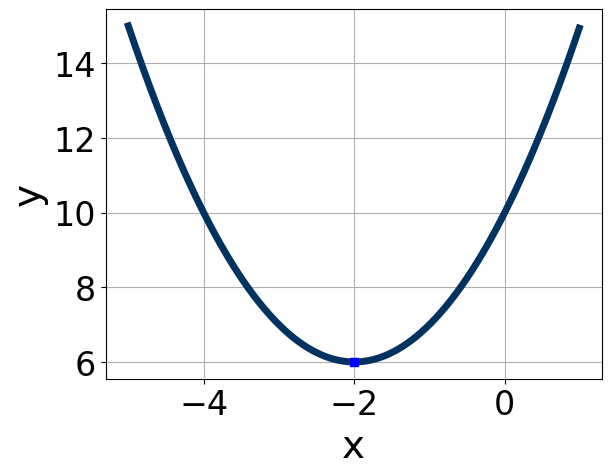
\includegraphics[width=0.5\textwidth]{../Figures/quadraticGraphToEquationCopyA.png}
\end{center}
\begin{enumerate}[label=\Alph*.]
\item \( a \in [0, 1.4], \hspace*{5mm} b \in [3, 5], \text{ and } \hspace*{5mm} c \in [9, 11] \)
\item \( a \in [0, 1.4], \hspace*{5mm} b \in [-4, 1], \text{ and } \hspace*{5mm} c \in [-2, 0] \)
\item \( a \in [0, 1.4], \hspace*{5mm} b \in [-4, 1], \text{ and } \hspace*{5mm} c \in [9, 11] \)
\item \( a \in [-1.2, -0.3], \hspace*{5mm} b \in [3, 5], \text{ and } \hspace*{5mm} c \in [0, 3] \)
\item \( a \in [-1.2, -0.3], \hspace*{5mm} b \in [-4, 1], \text{ and } \hspace*{5mm} c \in [0, 3] \)

\end{enumerate} }
\litem{
Graph the equation below.\[ f(x) = (x+4)^2 - 18 \]\begin{enumerate}[label=\Alph*.]
\begin{multicols}{2}\item 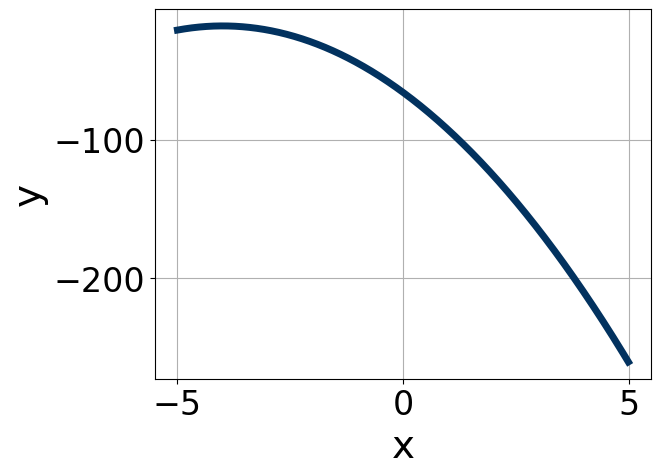
\includegraphics[width = 0.3\textwidth]{../Figures/quadraticEquationToGraphAA.png}\item 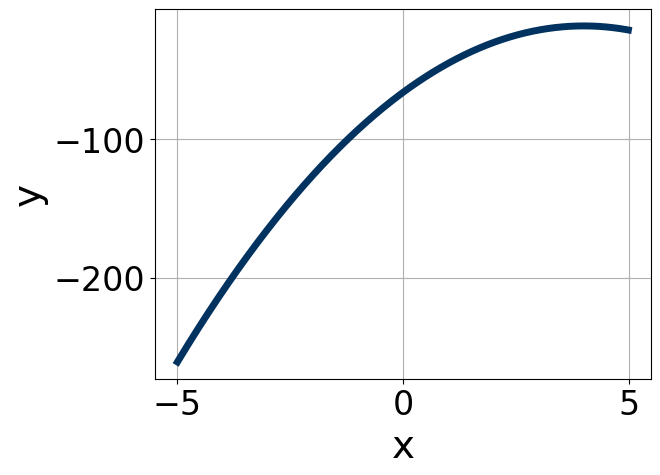
\includegraphics[width = 0.3\textwidth]{../Figures/quadraticEquationToGraphBA.png}\item 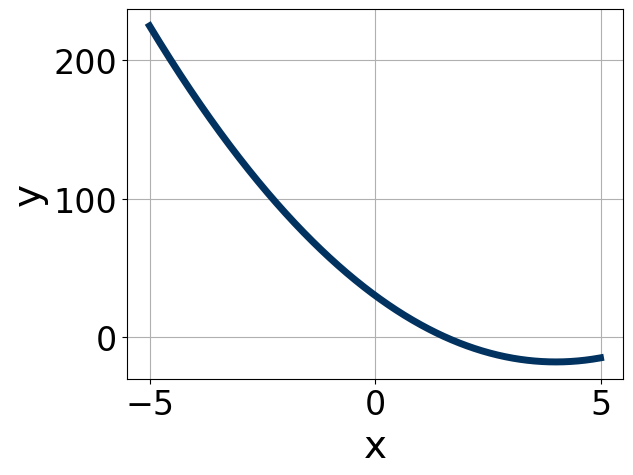
\includegraphics[width = 0.3\textwidth]{../Figures/quadraticEquationToGraphCA.png}\item 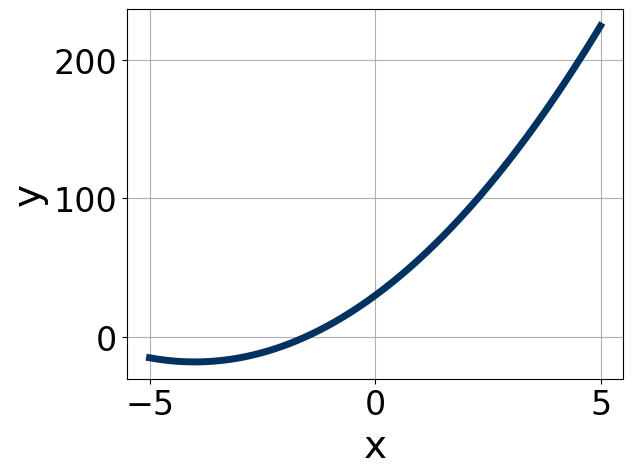
\includegraphics[width = 0.3\textwidth]{../Figures/quadraticEquationToGraphDA.png}\end{multicols}\item None of the above.
\end{enumerate} }
\litem{
Solve the quadratic equation below. Then, choose the intervals that the solutions $x_1$ and $x_2$ belong to, with $x_1 \leq x_2$.\[ 20x^{2} +21 x -54 = 0 \]\begin{enumerate}[label=\Alph*.]
\item \( x_1 \in [-9.03, -8.19] \text{ and } x_2 \in [0.16, 0.33] \)
\item \( x_1 \in [-7.24, -6.62] \text{ and } x_2 \in [0.31, 0.5] \)
\item \( x_1 \in [-3.06, -1.47] \text{ and } x_2 \in [1.19, 1.28] \)
\item \( x_1 \in [-45.82, -44.88] \text{ and } x_2 \in [23.87, 24.13] \)
\item \( x_1 \in [-1.66, -0.65] \text{ and } x_2 \in [3.46, 3.66] \)

\end{enumerate} }
\litem{
Factor the quadratic below. Then, choose the intervals that contain the constants in the form $(ax+b)(cx+d); b \leq d.$\[ 36x^{2} -60 x + 25 \]\begin{enumerate}[label=\Alph*.]
\item \( a \in [5.8, 7.1], \hspace*{5mm} b \in [-10, -3], \hspace*{5mm} c \in [3.5, 8.9], \text{ and } \hspace*{5mm} d \in [-8, -4] \)
\item \( a \in [0.3, 1.9], \hspace*{5mm} b \in [-30, -26], \hspace*{5mm} c \in [0.5, 2.4], \text{ and } \hspace*{5mm} d \in [-37, -24] \)
\item \( a \in [9.1, 15.3], \hspace*{5mm} b \in [-10, -3], \hspace*{5mm} c \in [2, 4.3], \text{ and } \hspace*{5mm} d \in [-8, -4] \)
\item \( a \in [1.1, 4.1], \hspace*{5mm} b \in [-10, -3], \hspace*{5mm} c \in [11, 13], \text{ and } \hspace*{5mm} d \in [-8, -4] \)
\item \( \text{None of the above.} \)

\end{enumerate} }
\litem{
Graph the equation below.\[ f(x) = (x+1)^2 - 17 \]\begin{enumerate}[label=\Alph*.]
\begin{multicols}{2}\item 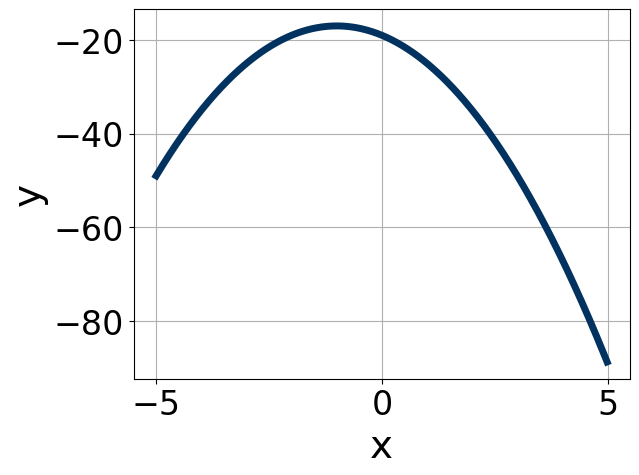
\includegraphics[width = 0.3\textwidth]{../Figures/quadraticEquationToGraphCopyAA.png}\item 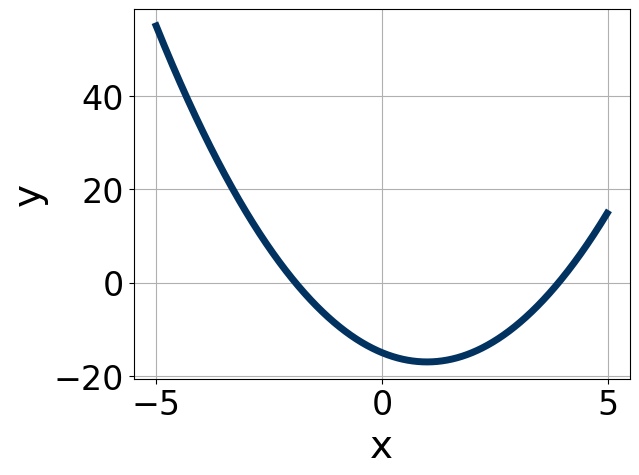
\includegraphics[width = 0.3\textwidth]{../Figures/quadraticEquationToGraphCopyBA.png}\item 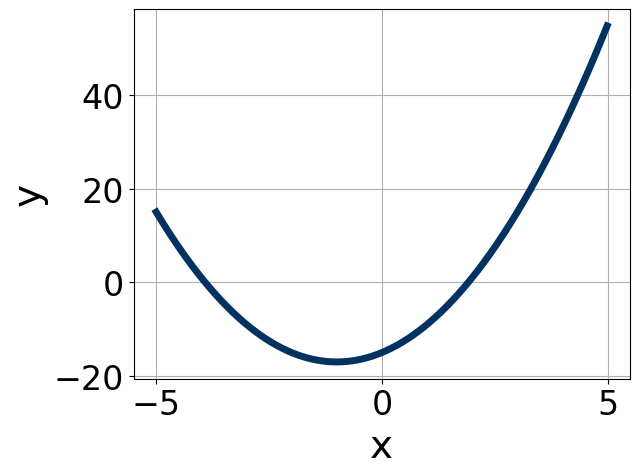
\includegraphics[width = 0.3\textwidth]{../Figures/quadraticEquationToGraphCopyCA.png}\item 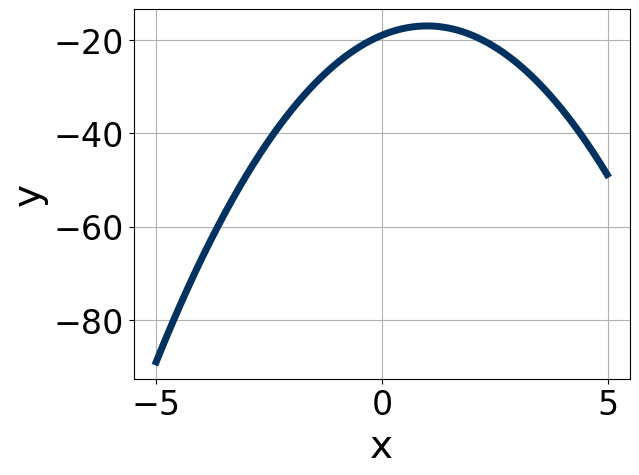
\includegraphics[width = 0.3\textwidth]{../Figures/quadraticEquationToGraphCopyDA.png}\end{multicols}\item None of the above.
\end{enumerate} }
\litem{
Solve the quadratic equation below. Then, choose the intervals that the solutions belong to, with $x_1 \leq x_2$ (if they exist).\[ 13x^{2} +14 x -2 = 0 \]\begin{enumerate}[label=\Alph*.]
\item \( x_1 \in [-0.8, 1.1] \text{ and } x_2 \in [0.93, 1.6] \)
\item \( x_1 \in [-16.6, -14.7] \text{ and } x_2 \in [1.66, 1.89] \)
\item \( x_1 \in [-3, -0.6] \text{ and } x_2 \in [-0.31, 0.41] \)
\item \( x_1 \in [-18, -16.5] \text{ and } x_2 \in [16.38, 17] \)
\item \( \text{There are no Real solutions.} \)

\end{enumerate} }
\litem{
Write the equation of the graph presented below in the form $f(x)=ax^2+bx+c$, assuming  $a=1$ or $a=-1$. Then, choose the intervals that $a, b,$ and $c$ belong to.
\begin{center}
    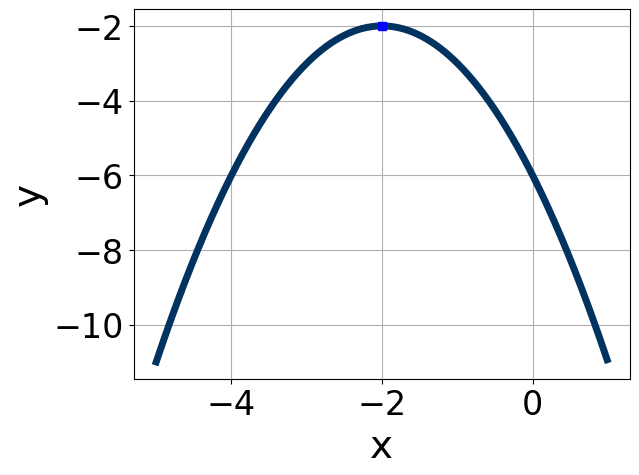
\includegraphics[width=0.5\textwidth]{../Figures/quadraticGraphToEquationA.png}
\end{center}
\begin{enumerate}[label=\Alph*.]
\item \( a \in [-0.2, 1.5], \hspace*{5mm} b \in [2, 6], \text{ and } \hspace*{5mm} c \in [2, 5] \)
\item \( a \in [-2.7, 0.9], \hspace*{5mm} b \in [-6, -2], \text{ and } \hspace*{5mm} c \in [-9, -5] \)
\item \( a \in [-0.2, 1.5], \hspace*{5mm} b \in [-6, -2], \text{ and } \hspace*{5mm} c \in [2, 5] \)
\item \( a \in [-2.7, 0.9], \hspace*{5mm} b \in [2, 6], \text{ and } \hspace*{5mm} c \in [-3, -1] \)
\item \( a \in [-2.7, 0.9], \hspace*{5mm} b \in [2, 6], \text{ and } \hspace*{5mm} c \in [-9, -5] \)

\end{enumerate} }
\end{enumerate}

\end{document}